\documentclass[linenumbers]{aastex631}
\usepackage[utf8]{inputenc}

\begin{document}
\title{Who is NGC2343...}
\author{Joaquin Stawsky}
\affiliation{San Diego State University \\
5500 Campanile Dr, \\
San Diego, CA 92182, USA}
\date{May 10, 2022}

\correspondingauthor{Joaquin Stawsky}
\email{jstawsky5784@sdsu.edu}

\begin{abstract}
We present a star cluster named NGC2343 at (107.025, -10.617) degrees in right ascension and declination. In this paper, we used data collected from the Mount Laguna Observatory's 1.0 meter telescope in the B and V band filters, data from the European Space Agency's Gaia mission, and the catalogue AAVSO Photometric All-Sky Survey (APASS). To understand the nature of NGC2343, we must use the queried data entailing celestial coordinates, parallax, and observed luminosities to deduce absolute magnitudes, distances, ages, and other important characteristics that could contribute to our understanding of the cluster's past and future. Throughout the study we conclude that the cluster as a whole lies at 1142.58 $\pm$ 90.21 parsecs from Earth, is between 10 and 100 million years old, and has a very low color excess value of 0.05. The cluster is very young, think that our Sun is about 4.5 billion years old, so NGC2343 will be around in the universe far longer than our star system will be. Starting after the data collection stage, an astronomer can follow the guidelines within this paper to accurately document our extra-solar neighborhood.
    
\end{abstract}


\section{Introduction}
As a result of their shared stellar origins, stars within clusters are relatively dense in population, have similar chemical compositions, and evolve in similar stages. Stars in a cluster have one main attribute that defines their evolutionary path beyond their cluster's characteristics: their individual, initial masses. The downside to mass having such an influence in stellar evolution is that one cannot exactly place a star on a scale. NGC2343 is an open cluster of stars in the Monoceros constellation, and as such, the cluster is ideal for comparing to isochrones of stellar clusters. Given their celestial coordinates, respective proper motions, parallax, and observed luminosities, a person will be able to make many inferences about the cluster's past, present, and future.

Calculating the distance, estimating the age, and measuring the excess color of a star cluster are all essential steps in defining the characteristics that make each cluster unique. The distances provide necessary information to calculate the velocity of galaxies, stars, and clusters using Hubble's Law. Ages, along with observed and absolute luminosities, of celestial objects allow astronomers to make inferences about these objects' evolution: their initial masses and their ultimate fates. It is also important to note that to properly estimate a star's age, one should also observe the star's surroundings since most members of a group of stars will be coeval. Defining the ever-positive excess color value of celestial objects, denoted by E(B-V), can help an astronomer determine how much light received is actually part of the desired object and not from the interstellar medium. In turn, the excess color calculation provides information about interstellar absorption quantities as well as galactic extinction ratios, both varying depending on where the observer is looking. When observing NGC2343, and other star clusters in general, one has the opportunity to test the models of stellar evolution.

Using data from Mount Laguna Observatory's 1.0 meter telescope, Gaia
\footnote{This work has made use of data from the European Space Agency (ESA) mission {\it Gaia} (\url{https://www.cosmos.esa.int/gaia}), processed by the {\it Gaia} Data Processing and Analysis Consortium (DPAC, \url{https://www.cosmos.esa.int/web/gaia/dpac/consortium}). Funding for the DPAC has been provided by national institutions, in particular the institutions participating in the {\it Gaia} Multilateral Agreement.} 
mission's legendary sky survey, and the AAVSO Photometric All-Sky Survey (APASS) from \citep{2016yCat}, we were able to conduct astrometric and photometric analyses, create a Color Magnitude Diagram (CMD), and approximate the cluster's age. In Section \ref{data}, we describe the photometric, astrometric, and image data collected. In Section \ref{analysis}, we address how we produce the model comparisons, using the data collected. In Section \ref{conclusions}, we compile the information and results reached throughout the process. 

\section{Data}\label{data}
%talk about NGC: origins and current surveys used
We begin the study using image data taken from the Mount Laguna Observatory (MLO). Specifically, this entails images taken with the B and V band filters at differing exposure times (5, 20, 80 seconds), 25 bias images, and six twilight pictures taken for each filter. The advantage in taking images in the B and V bands lies in having a relatively wide range of optical wavelengths for comparison; choosing shorter exposure times allows for brighter stars to be observed accurately and longer times for dimmer objects. Since bias images are used to remove electronic noise generated by the Charge Coupled Device (CCD), most of them are taken with low exposure times, far less than one second, and usually in quantities of 25 to 100 total images to find an average that describes the pixels in the CCD accurately. Flat field images are used to properly account for the fluctuations in sensitivity to light on a CCD's pixels as well as smudges or dust caught in the telescope. These images are also referred to as twilight images because the light in the sky is uniform; to get a good flat an astronomer must aim for the most uniform amount of light receivable across the CCD. In astronomy, and most other sciences, it is useful to compare or use data that was not taken by you.

The Gaia archive was used to collect data describing right ascension (R.A.), declination (Dec.), proper motion in both axes, and the parallax angle along with its error. Calculating the distance to these celestial objects is as simple as $$d = \frac{1}{p}$$ such that $p$ denotes the parallax measured in arcseconds and $d$ is the distance in parsecs. Additionally, we took data from the APASS catalogue to cross-reference with our Gaia data and contribute the observed magnitudes of each object's luminosity in the B and V bands. These two queries are matched by their R.A. and Dec. with the MLO B and V filter data to convert the counts from the CCD into observed magnitudes. Comparing the different sources of data, we can define a stars membership in the NGC2343 cluster by the distances and proper motion distributions. As the last group of data utilized, isochrone models serve the purpose to compare our processed MLO data to known evolutionary models that are characteristic for different ages \citep{2012MNRAS.427..127B}. An important possible source of inaccuracy to consider are the parameters defining a stars membership to the cluster. The errors in the calculations of distance, counts in the CCD, and magnitudes of each band are possible sources of imprecision as well. That being said, the likelihood of getting inaccurate results decreases with the cross-referencing of different sources of data.

\section{Analysis}\label{analysis}
Before one can call an image 'processed', they should first remove the overscan region used for addressing small variations in the pixels, subtract the master bias frame (an average of the 25 individual bias images), and divide by the flat field images in each band filter. Each overscan, bias, flat, and image processing step has their own referable function. We continue to define NGC2343's location by its given R.A. and Dec. (107.025, -10.617) in degrees, query Gaia using the Astronomical Data Query Language (ADQL), and plot the group of objects collected: Figure \ref{fig:gaia}. Using the APASS catalogue, we collect the observed B and V band magnitudes, adding it into a data multi-dimensional array with the Gaia data. Once both queries have been made, we match them by their coordinates with a separation of less than 2 arcseconds in the R.A. and Dec., matching results are plotted in Figure \ref{fig:match}.
\begin{figure}
    \centering
    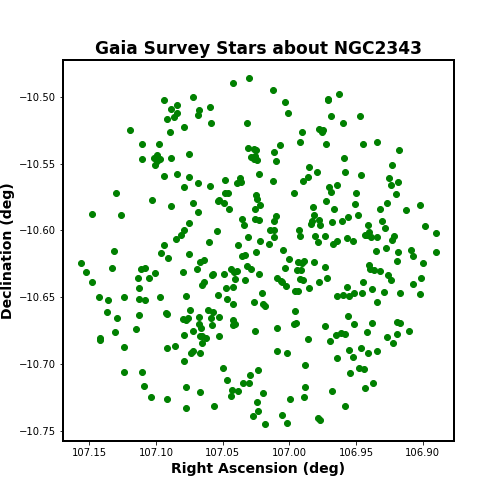
\includegraphics[scale = 0.5]{pngs/Gaia_Survey_Stars_about_NGC2343.png}
    \caption{\label{fig:gaia} The known coordinates for NGC2343 are at the center of this plot, with other celestial objects that have similar right ascensions and declinations within 8 arcminutes of the clusters.}
    \label{fig:gaia}
\end{figure}
\begin{figure}
    \centering
    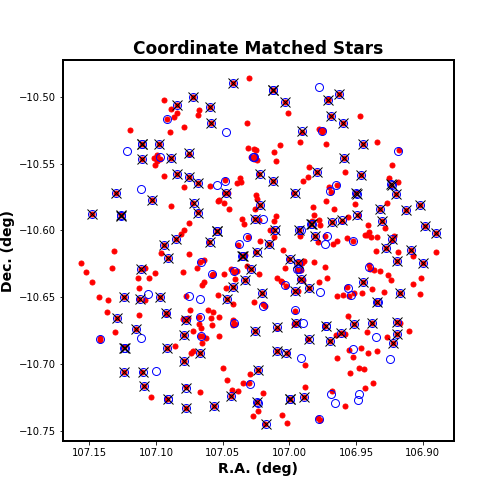
\includegraphics[scale = 0.5]{pngs/coordinates_matched.png}
    \caption{\label{fig:match} Similar to \ref{fig:gaia}, this plot contains the data collected from Gaia (red circles) and matches it with data from the APASS catalogue (blue, empty circles). A match in coordinates is displayed as a blue X containing both blue and red circles within.}
    \label{fig:match}
\end{figure}

We define one function to get the counts of photons within a specified, small, circular aperture whose radius is defined by the file's full width half maximum value (FWHM). FWHM is a measure of sharpness in the image, dependant on how far the telescope and atmosphere blur a single object's light across the CCD's pixels. The other important function used in this step calculates the photometry of each B or V band image (6 total). This function references the counts function mentioned above to calculate the zero-point magnitude of each image and ultimately the observed magnitude of each object in the figure. The magnitudes calculated, and their uncertainties, are added to the data file containing the rest of the Gaia and APASS data. The color, defined by the magnitude in the B band subtracted by the magnitude in the V band, is plotted versus the V band magnitude taken from the function referenced above: Figure \ref{fig:CMD}. Processing the images and conducting the photometric analyses is essential to our conclusions, but deemed useless if we cannot properly define what it means to be a member of the cluster NGC2343. 
\begin{figure}
    \centering
    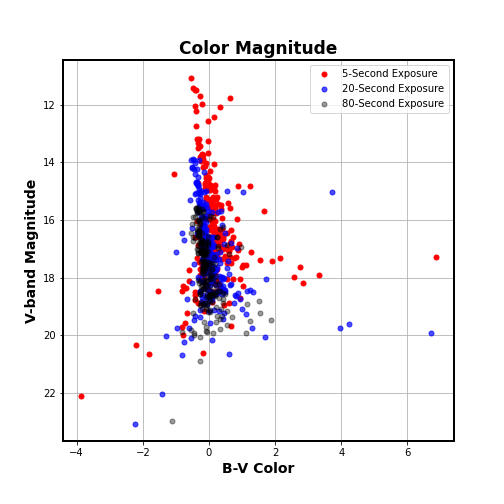
\includegraphics[scale = 0.5]{pngs/CMD_5_20_80.png}
    \caption{\label{fig:CMD} Shown above is the Color Magnitude Diagram for the data collected by MLO's telescope, differentiating the dimmest stars in 80-second exposures from the brightest with the 5-second exposures.}
    \label{fig:CMD}
\end{figure}

Using the distance calculated and proper motions measured from the Gaia data, we plot and create parameters that differentiate the cluster's members from background light sources, Figure \ref{fig:histo}. Distance for the parameters were defined to be one standard deviation above and below the median distance calculated, the range is from 458.96 to 1826.21 parsecs from Earth. The parameters for proper motion in right ascension and declination were also defined as being within one standard deviation above or below the median, Figure \ref{fig:pm}. By this point, the data was already constrained to be within the distance's parameters of membership. Median values were used in both calculations instead of mean values as a definition of the cluster's center as a result of the median being more resistant to outliers than the mean. In R.A., the proper motion values should lie between -3.32 and 3.45 milliarcseconds per year; in Dec. the proper motion values should lie between -5.44 and 5.09 milliarcseconds per year.
\begin{figure}
    \centering
    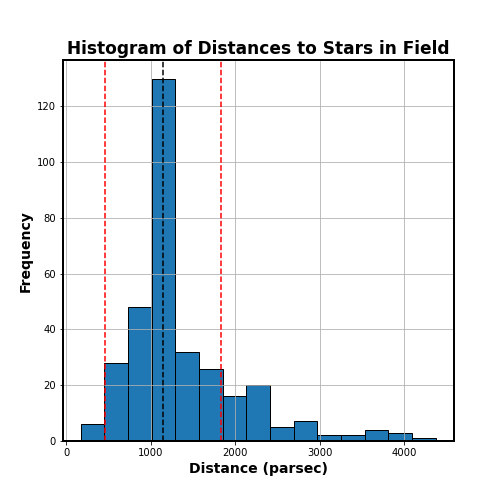
\includegraphics[scale = 0.5]{pngs/hist_to_dists.png}
    \caption{\label{fig:histo} The histogram of the distances to all the stars within the radius of observation are depicted, with the black, dashed line being the median of the distances and the red, dashed lines establishing one standard deviation above and below the median.}
    \label{fig:histo}
\end{figure}
\begin{figure}
    \centering
    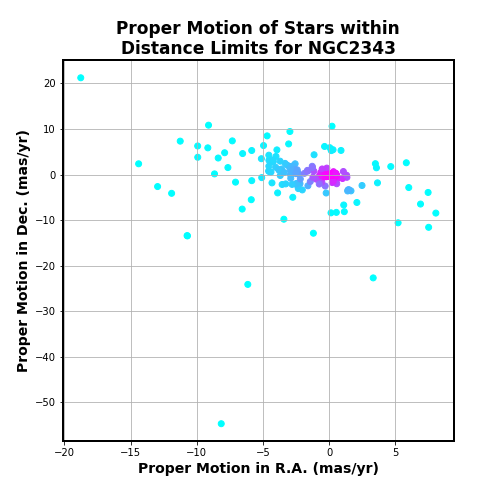
\includegraphics[scale = 0.5]{pngs/proper_motion_in_dists.png}
    \caption{\label{fig:pm} The proper motions of each star within the distance parameters are shown with the population density being the most at the purple points.}
    \label{fig:pm}
\end{figure}

Beyond solely being part of the cluster, we must also account for the light contamination from other objects in the celestial vicinity by first identifying the objects in our data that are isolated. The criteria for an isolated star in this case is that there are no other objects within 10 arcseconds from its location. We continue to load the model data from \citet{2012MNRAS.427..127B} to compare the model with the data collected using the $\chi^{2}$ method. The model is split into three sections, defined by their respective ages: Figure \ref{fig:iso7}, \ref{fig:iso8}, \ref{fig:iso9}. The $\chi^{2}$ method entails using calculated data to see which points from the model it is closest to. At this point, we further constrain the data such that we only include stars if they are members of the cluster, are isolated, and have values for B and V absolute magnitudes. Thus, we show the results in Figure \ref{fig:model}.

\begin{figure}
    \centering
    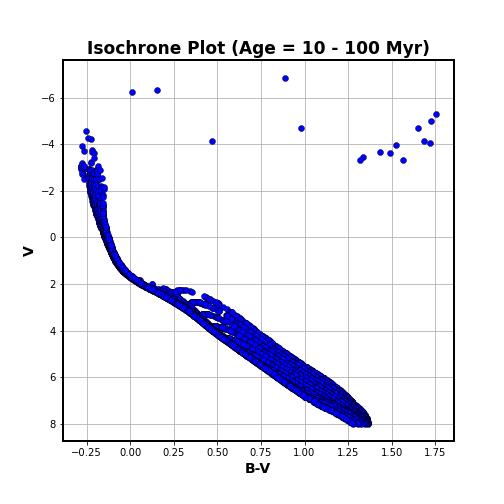
\includegraphics[scale = 0.5]{pngs/iso7.png}
    \caption{\label{fig:iso7} The model isochrone data is displayed for stars with ages between 10 and 100 million years.}
    \label{fig:iso7}
\end{figure}
\begin{figure}
    \centering
    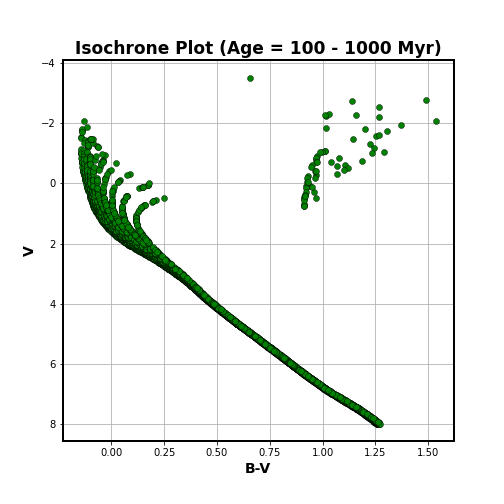
\includegraphics[scale = 0.5]{pngs/iso8.png}
    \caption{\label{fig:iso8} The model isochrone data is displayed for stars with ages between 100 million and 1 billion years.}
    \label{fig:iso8}
\end{figure}
\begin{figure}
    \centering
    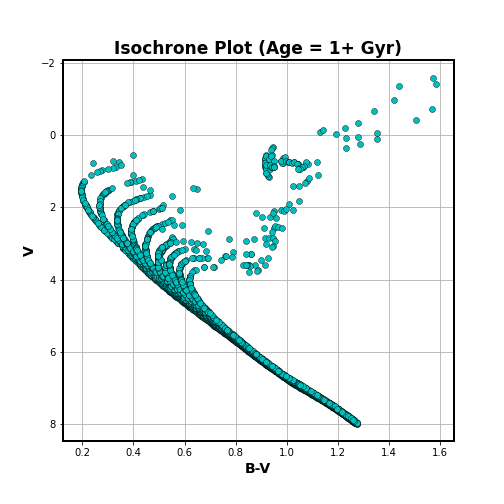
\includegraphics[scale = 0.5]{pngs/iso9.png}
    \caption{\label{fig:iso9} The model isochrone data is displayed for stars with ages over 1 billion years.}
    \label{fig:iso9}
\end{figure}

\begin{figure}
    \centering
    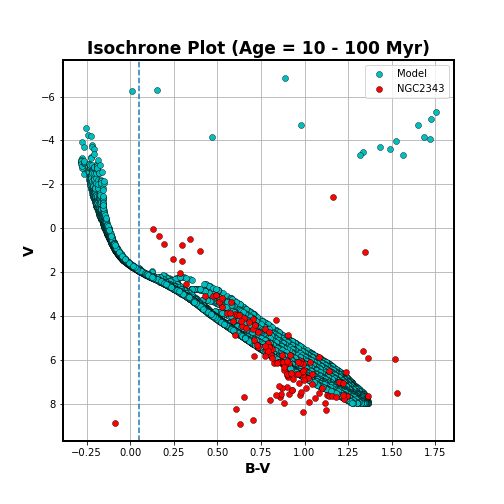
\includegraphics[scale = 0.5]{pngs/model_fit.png}
    \caption{\label{fig:model} Compared to Figure \ref{fig:iso7}, the final data set (red) portrays very similar characteristics. The vertical, blue, dashed line represents the calculated E(B-V) for the cluster. }
    \label{fig:model}
\end{figure}

\section{Conclusions}\label{conclusions}
In describing NGC2343, we can now describe it using our own calculated values for distance, approximate age, and excess color. The calculated, median distance of all the stars in the cluster is 1142.59 parsecs. NGC2343 is a relatively young star cluster, its age is between 10 and 100 million years. The cluster's color excess (0.05) is very low, most likely caused by there not being much light interference. This paper described, and displayed, the relationship between luminosity and color. Within this relationship, we exemplified the impact that the age of a star or cluster has on its color and magnitude, and the inferences that one could make about the object's initial mass. 
Although the results of this study are accurate, possible limitations to this methodology lie in the fact that we were only able to use 131 values to describe the cluster in the end. There exists more members within NGC2343 but limitations in telescopes and our perspective as a result of our place in the universe can cause us to lose some stars that are hidden or too dim. Using more celestial surveys/catalogues could incorporate other stars that were missed by APASS and Gaia. Additionally, using data other than that from MLO could provide more accurate results and having different band-pass filters could prove beneficial.


\bibliography{final}{}
\bibliographystyle{aasjournal}
\end{document}
